\section{Stream Processing and its Building blocks}

\subsection{Background}

\begin{figure}[h]
	\centering
	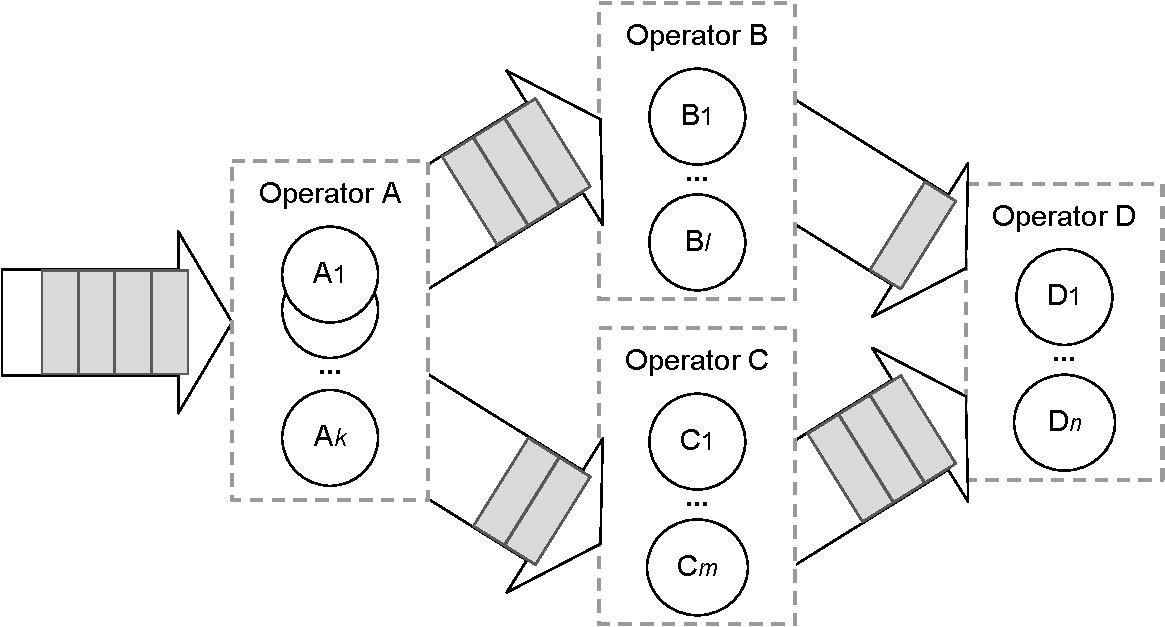
\includegraphics[width=0.6\linewidth]{stream.pdf}
	\caption{Conceptual overview of stream processing.}
	\label{fig:stream}
\end{figure}

This section clarifies the terminology used in this article. Both the research and industry community have independently developed various stream processing frameworks, each with their own terminology and model. While there are differences, both at the language level and at the
system level, we use a generalized and abstract terminology derived based on \cite{optimization-survey}.

A stream \textit{application} is represented as a directed graph called a \textit{dataflow}. In this graph, each vertex is an operator and each edge is a stream of data, as shown in Figure \ref{fig:stream}.
A \textit{stream} is an infinite sequence of data \textit{items}. Streams behave similar to queues -- items are processed from the front and new items are added to end.

An \textit{operator} is a continuous stream transformation. An operator handles an arbitrary non-negative number ($\geq 0$) of input streams and output streams. Each operator, consumes items from it incoming stream(s) one at a time; performs computation and transformation on the item; and optionally generates one or more new items into an output stream(s). Thus, streams connect operators and make the data flow through the dataflow while operators perform the transformations on the data. 
Each operator has a number of \textit{instances}, e.g. $\{A_1, ..., A_k\}$ of operator A in Figure \ref{fig:stream}. In parallel, each instance, e.g. $A_i$, performs the exact same computation but on a separate portion of the input stream(s).

 

\Fix{Do we need an example here?}
\Fix{should we talk about 1.when data is generated/outputted?2. buffers 3.state, 4. distribution}


\begin{itemize}
	\item basic definitions of stream processing. 
	\item what is operator
	\item how do messages flow
	\item how operators are connected
	\item API
\end{itemize}





\subsection{High Level Overview}
\begin{itemize}
	\item describe the main building blocks. These are in Table \ref{table:blocks}
	\item discuss the definition, purpose, importance of each block.	
\end{itemize}


\begin{table}[h]
	%\centering
	\tbl{Essential building blocks in Stream Processing Engines.	\label{table:blocks}}{
		\begin{tabular}{c|l|l|c}%
			\hline
			\rowcolor[HTML]{E0E0E0} 
			\bfseries Section & \bfseries Building Block & \bfseries Definition & By % specify table head
			\csvreader[head to column names]{tables/building-blocks.csv}{}% use head of csv as column names
			{\\\hline\csvcoli&\csvcolii & \csvcoliii & \csvcoliv}% specify your coloumns here
			\\ \hline
		\end{tabular}
	}
\end{table}

\Fix{Do we want to argue we are covering all essential building blocks??? or just say the most important ones?}
\Fix{ should we talk about ordering somewhere? which BB does it belong to?}
\Fix{Where does lenght of processing fall (Independent msg,
	Window based processing,
	Infinite data)}



\subsection{Interaction Among Building Blocks}

\begin{itemize}
	\item Draw a figure of the building blocks and their interaction. 
	\item Talk about how the influence each other
	\item Maybe try to break them down into a layers? with some being in a touching-all layer?
\end{itemize}


%

\begin{figure}[h]
	\centering
	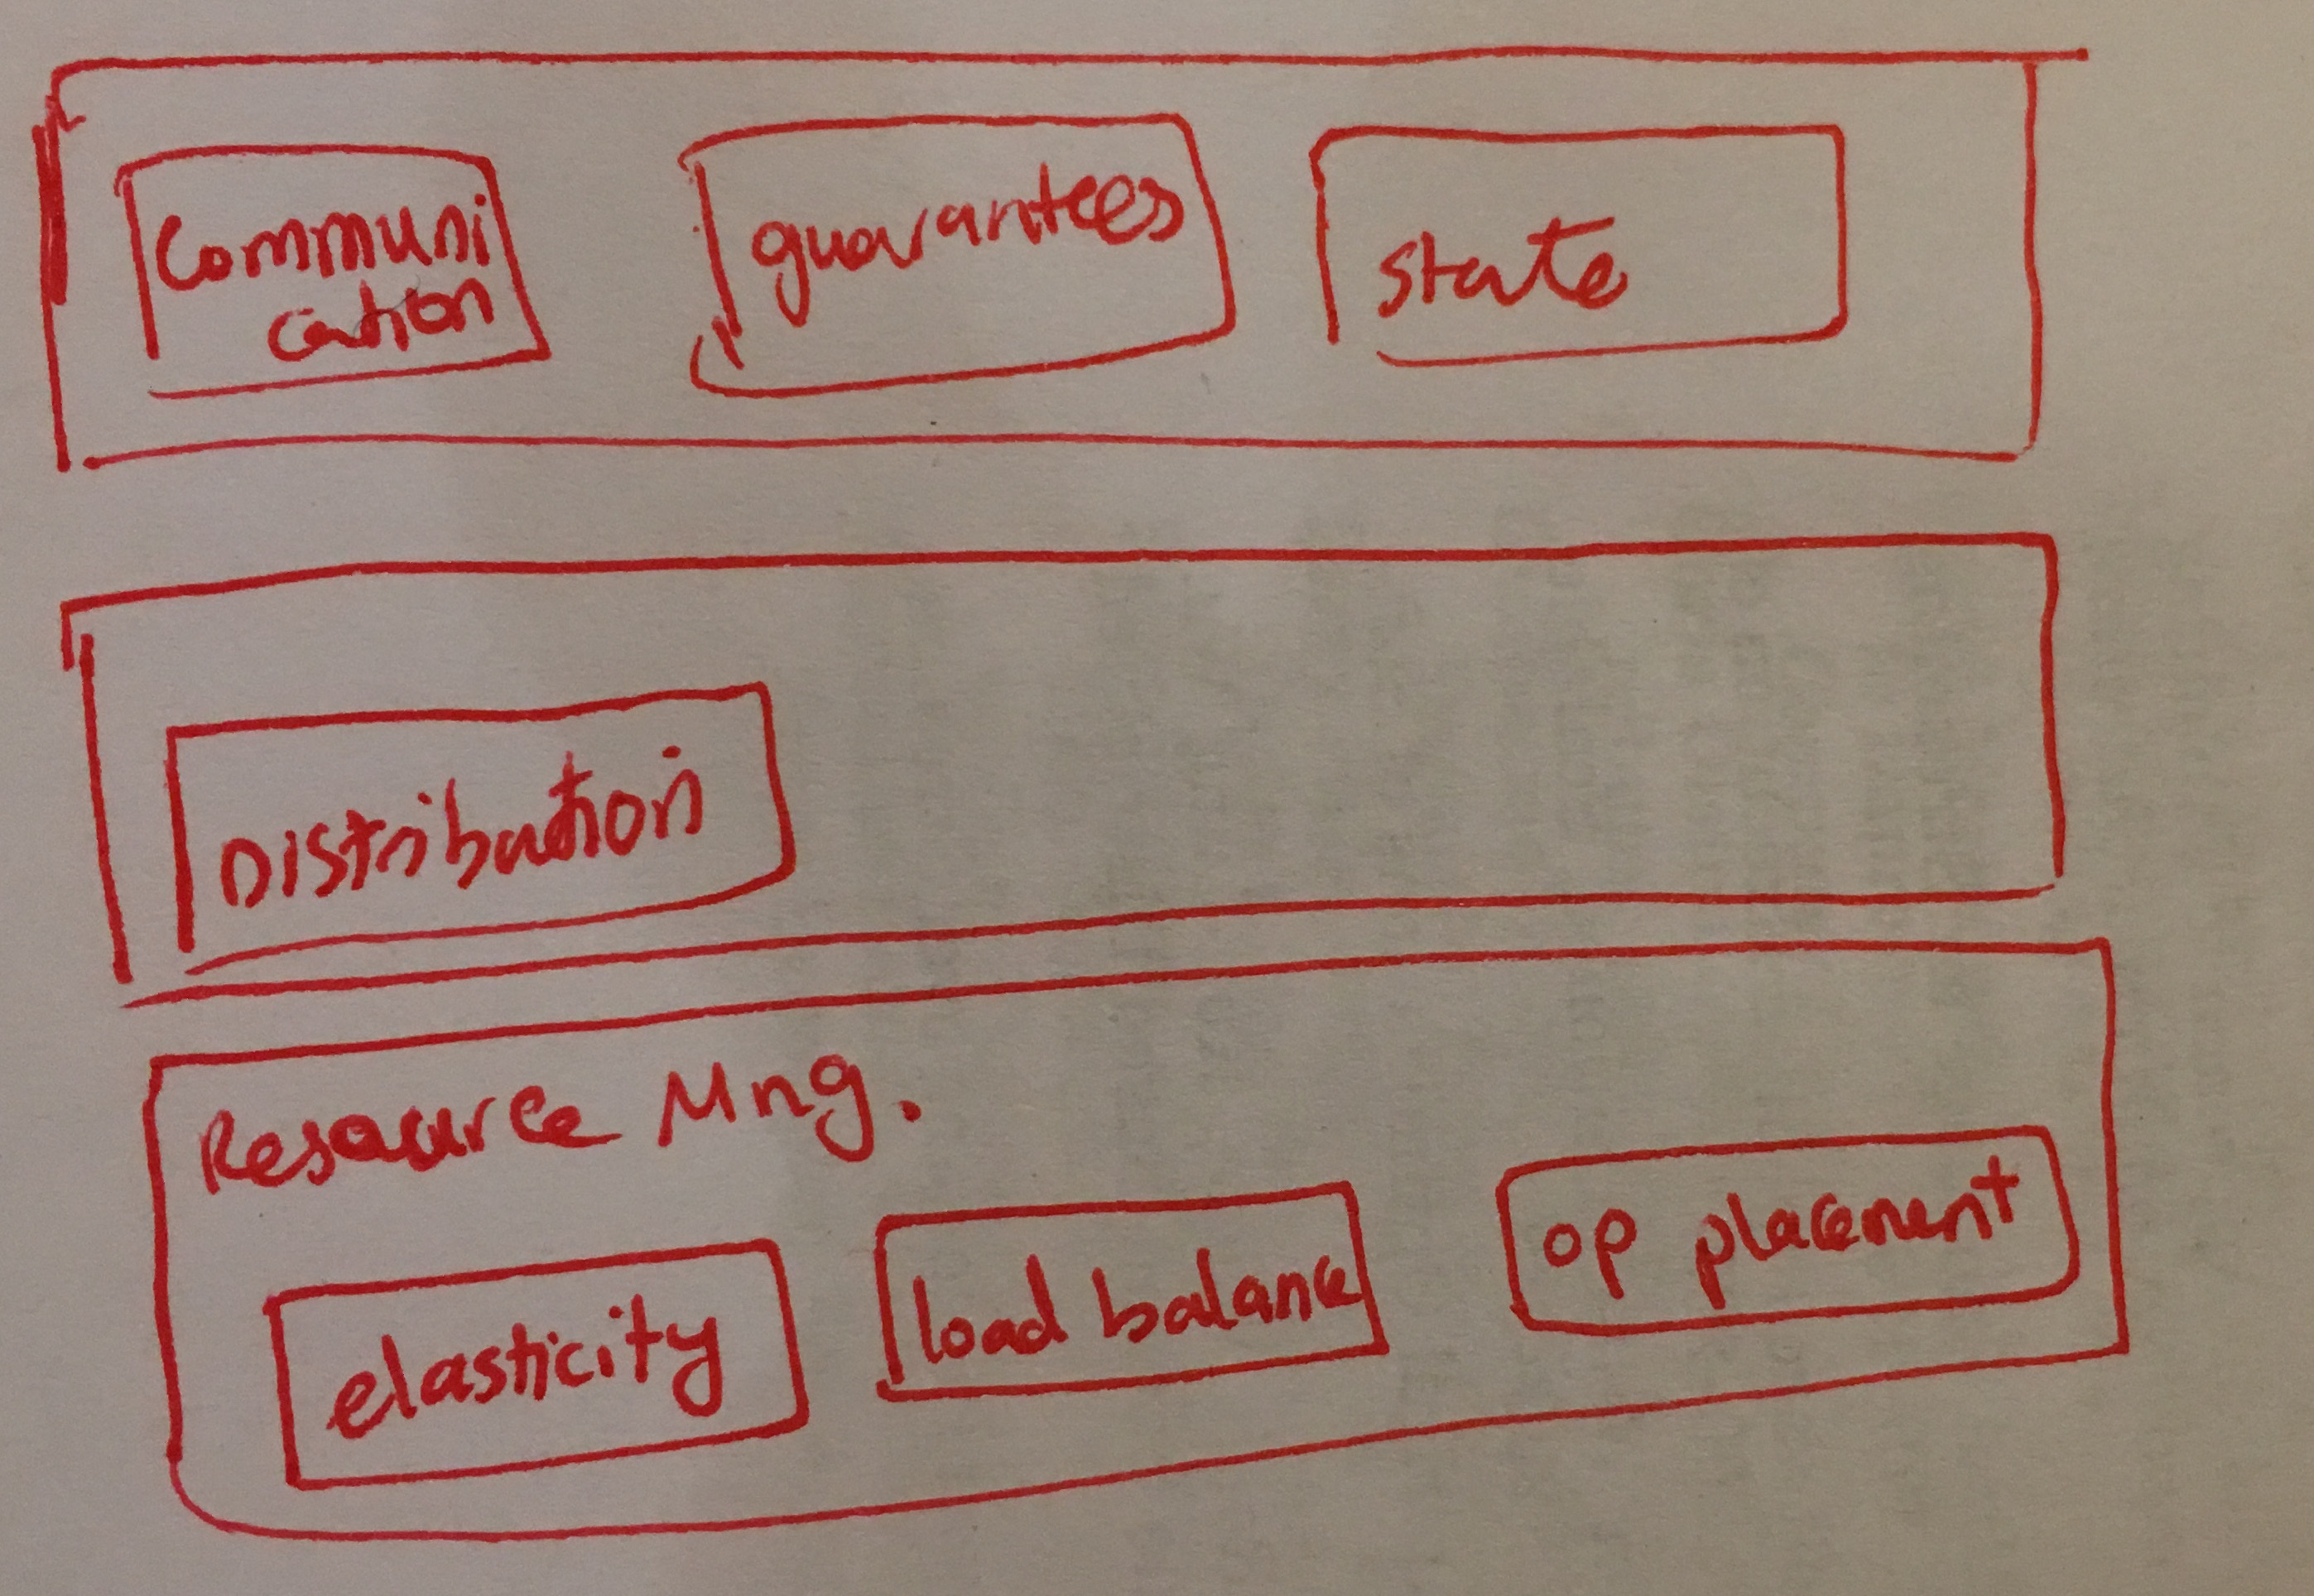
\includegraphics[width=0.45\linewidth]{interaction.jpg}
	\caption{\Fix{Sample figure of how components interact with one another. This is not complete.}}
	\label{fig:tree-cpVScl}
\end{figure}


